\documentclass[article]{IEEEtran}
\usepackage[utf8]{inputenc}
\usepackage[pdftex]{graphicx}
\graphicspath{./}

\begin{document}

\title{Motor de passo}

\author{Danilo Souza, Hugo Santos, Welton Ara\'ujo

%\thanks{Engenharia da Computa\c{c}\~ao, Universidade Federal do Par\'a, Bel\'em-PA, Brasil}
Emails: \{dhcsouza, hugoleonardoeng07, weltonmaxx007\}@gmail.com\\
Matr\'iculas: 10080000801, 10080000701, 10080000501}

\maketitle

\begin{abstract}
There is a lot of possibilities to do with microcontrollers because they are very flexible. This project implements a stepper motor program which switches between clockwise direction and counter clockwise direction. Beyond this, it switches between three different types of steps. The code was made on machine language, in other words Assembly with specifics instructions for the PIC16F877A. This PIC has several limitations, but could perfectly attend the game requirements in this case.
\end{abstract}

\begin{IEEEkeywords}
microcontroller, PIC16F628, game, shock, multiplayer
\end{IEEEkeywords}

\IEEEpeerreviewmaketitle


\section{Introduçao}
O PIC16F877A faz parte da família PIC de microcontroladores da Microchip Technology, composta também por diversos outros modelos, como o PIC16F873A, PIC16F874A e PIC16F876A que diferem, por exemplo, na	capacidade de memória flash disponível para armazenamento de programas.

A família PIC é amplamente utilizada hoje em dia devido a sua facilidade de programação e uma grande documentação disponível, suas aplicações podem variar desde simples protótipos até automação industrial, sua flexibilidade garante sua utilização em praticamente qualquer indústria.

A partir disto, o projeto abordado neste artigo aproveitou a possibilidade de utilizar correntes de até 200mA diretamente para alimentar  as bobinas de um motor de passo.

\section{Descrição do Projeto}
O projeto baseia-se em um motor de passo de quatro bobinas. Essas são ligadas de tal forma que faz o eixo do motor girar com torque, velocidade e posicionamento definidos pelo tipo de passo indicado e da temporizaçao.

Existe três tipos de passo distintos, são eles:
\begin{itemize}
	\item \textbf{Simples 1}: o motor gira de 90 em 90 graus onde o rotor do motor direciona-se para a bobina energizada.
	\item \textbf{Simples 2}: o motor também gira de 90 em 90 graus, porém duas bobinas adjacentes são ligadas simutaneamente fazendo com que o rotor direcione-se entre as duas bobinas energizadas, nesta forma existe um ganho de torque em relaçao ao simples 1.
	\item \textbf{Meio-passo}: motor gira de 45 em 45 graus de um forma em que os passos simples 1 e simples 2 se misturam, isto é, durante o giro do motor são ligados uma ou duas bobinas adjacentes fazendo com que o motor gire somente 45 graus.
\end{itemize}

No começo o motor inicia utilizando o passo simples 1 no sentido horário. O botão de sentido faz com que seja invertido o sentido de rotaçao do eixo do motor. O botão de passo alterna entre os três tipos de passos.
 
\section{Funcionamento do Programa}
O algoritmo de funcionamento do programa funciona com o auxílio das variáveis da Tabela \ref{tab:variaveis} onde também são descritas suas funções de controle. A Tabela \ref{tab:bits} contém os pinos do PIC utilizados como saídas e entradas juntamente com suas funções. A Figura \ref{fig:fluxograma} mostra o fluxograma das rotinas  mais determinantes do código.

\begin{figure}	
		\centering
		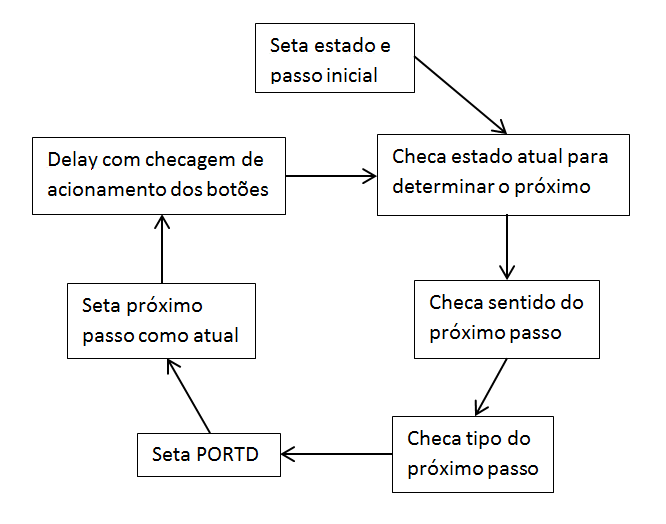
\includegraphics[width=8.5cm]{./fluxograma.png}
		\caption{Fluxograma do programa}
 		\label{fig:fluxograma}
\end{figure}

Inicialmente, o programa começa pré-configurado para rodar no sentido horário com o passo simples 1 também setado para iniciar a partir do estado e passo 1. Um atraso faz com que as bobinas sejam acionadas durante um certo tempo para, em seguida, a próxima ser acionada. Caso o botão de sentido seja apertado, instaneamente será setado o estado anterior sem que haja espera no \textit{delay}, isto é, o tempo de resposta ao botão é quase imperceptível.

Outro botão existente é responsável pela mudança entre os tipo de passo. O programa definiu o ciclo na ordem simples 1, simples 2 e meio passo. Neste botão também o tempo de resposta é quase imperceptível, pois rapidamente é buscado setar as bobinas do tipo de passo escolhido para o próximo estado considerando também o sentido.

Os botões somente cumprem a sua função quando há o despressionamento do mesmo, pois dessa forma previne-se que a escolha de sentido e passo seja aleatória. Isso acontece porque o botão entre em um laço esperando que seu valor tenha nível lógico baixo.

É importante ressaltar que a responsividade rápida aos comandos dos botões acontece porque eles são checados durante os laços do \textit{delay}, pois o programa roda a maior parte do tempo nas rotinas responsáveis por este atraso.

A Tabela \ref{tab:variaveis} contém as variáveis de controle utilizadas com suas descrições. A Tabela \ref{tab:rotinas} contém as principais rotinas com suas descrições. A Tabela \ref{tab:bits} contém as sequências de bits utlizadas durante o programa para selecionar estados, passos e valor dos contadores.

\begin{table}
  \centering
  \caption{Variáveis de controle}
  \vspace{0.5cm}
  \label{tab:variaveis}
  \begin{tabular}{|p{2cm}|p{1cm}|p{3.3cm}|} \hline
    Variáveis 	& Endereco & Descrição 						\\ \hline
    REG			& 0x20	   & bit 0 determina sentido e os bits 1,2 e 3 o tipo de passo			\\ \hline
    CUR\_STATE	& 0x21	   & Estado atual de energizaçao das bobinas		\\ \hline  
    COUNT1		& 0x22	   & Contador 1 para o delay para alternar de estado	\\ \hline
    COUNT2		& 0x23	   & Contador 2 para o delay para alternar de estado	\\ \hline
    COUNT3		& 0x24	   & Contador 3 para o delay para alternar de estado	\\ \hline
  \end{tabular}
\end{table}

\begin{table}
  \centering
  \caption{Rotinas - X varia de 1 a 8}
  \vspace{0.5cm}
  \label{tab:rotinas}
  \begin{tabular}{|p{3cm}|p{4.3cm}|} \hline
    Rotina				& Descrição 					\\ \hline
    CHECK\_CUR\_STATE  	& Checa o estado atual do motor	\\ \hline
    STATEX\_OPT			& Checa qual será o próximo estado de acordo com o sentido							\\ \hline
    CW\_STATEX			& Checa qual será o tipo de passo do passo em questão no sentido horário 		\\ \hline
	CCW\_STATEX			& Checa qual será o tipo de passo do passo em questão no sentido anti-horário	\\ \hline
    S1\_SET\_STATEX		& Seta o estado X em CUR\_STATE, o passo X no PORTD com o passo tipo simples 1, dá o \textit{delay} e vai para a rotina de checar o estado atual 							\\ \hline
	S2\_SET\_STATEX		& Seta o estado X em CUR\_STATE, o passo X no PORTD com o passo tipo simples 2, dá o \textit{delay} e vai para a rotina de checar o estado atual							\\ \hline    
  \end{tabular}
\end{table}


\begin{table}
  \centering
  \caption{Bits de controle}
  \vspace{0.5cm}
  \label{tab:bits}
  \begin{tabular}{|p{2.3cm}|p{5cm}|}\hline
    Bits 			& Descrição						\\ \hline
    DIR\_BUTTON		& Botão no bit 0 do PORTD para mudar o sentido de rotaçao do motor	 \\ \hline
    STEP\_BUTTON	& Botão no bit 1 do PORTD para mudar o tipo de passo do motor	     \\ \hline
    STEP1			& Valor que será setado no PORTD	para setar o passo 1 \\ \hline
	STEP2			& Valor que será setado no PORTD	para setar o passo 2 \\ \hline
	STEP3			& Valor que será setado no PORTD	para setar o passo 3 \\ \hline
	STEP4			& Valor que será setado no PORTD	para setar o passo 4 \\ \hline
	STEP5			& Valor que será setado no PORTD	para setar o passo 5 \\ \hline
	STEP6			& Valor que será setado no PORTD	para setar o passo 6 \\ \hline
	STEP7			& Valor que será setado no PORTD	para setar o passo 7 \\ \hline
	STEP8			& Valor que será setado no PORTD	para setar o passo 8 \\ \hline
	STATE1			& Valor que será memorizado na variável CUR\_STATE quando o estado for 1 \\ \hline
	STATE2			& Valor que será memorizado na variável CUR\_STATE quando o estado for 2 \\ \hline
	STATE3			& Valor que será memorizado na variável CUR\_STATE quando o estado for 3 \\ \hline
	STATE4			& Valor que será memorizado na variável CUR\_STATE quando o estado for 4 \\ \hline
	STATE5			& Valor que será memorizado na variável CUR\_STATE quando o estado for 5 \\ \hline
	STATE6			& Valor que será memorizado na variável CUR\_STATE quando o estado for 6 \\ \hline
	STATE7			& Valor que será memorizado na variável CUR\_STATE quando o estado for 7 \\ \hline
	STATE8			& Valor que será memorizado na variável CUR\_STATE quando o estado for 8 \\ \hline
	D1				& Valor para ser setado em COUNT1 \\ \hline
	D2				& Valor para ser setado em COUNT2 \\ \hline
	D3				& Valor para ser setado em COUNT3 \\ \hline
  \end{tabular}
\end{table}

\section{Simulaçao}
A simulaçao foi feita no \textit{software} Proteus, o circuito lá montado buscava somente simular o funcionamento do projeto da forma mais simples e clara possíveis. Portanto, não foram adotados circuitos de proteção para o funcionamento idêntico ao do projeto de \textit{hardware}. 

A Figura \ref{fig:simulacao} mostra que os pinos do motor foram ligados nas portas RD2, RD3, RD4 e RD5 do PORTD. Os botões foram ligados no pinos RD0 e RD1, também do PORTD.

	\begin{figure}	
		\centering
		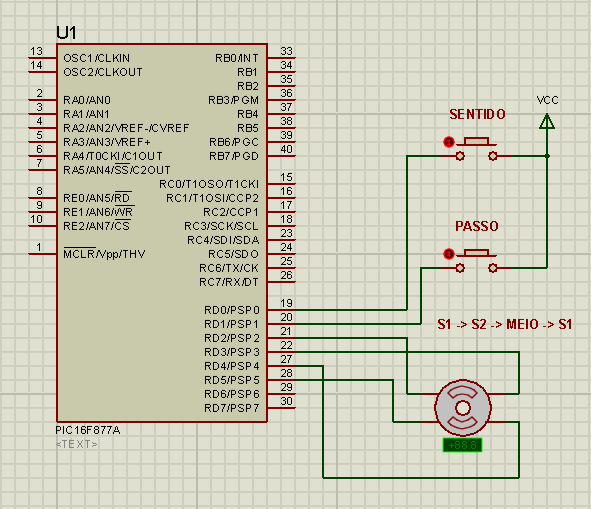
\includegraphics[width=8.5cm]{./simulacao.png}
		\caption{Simulaçao no Proteus}
 		\label{fig:simulacao}
	\end{figure}

\section{Conclusão}
A utilizaçao da linguagem de programação Assembly forneceu as maiores dificuldades para o grupo concluir o projeto. Percebeu-se que o código ficou relativamente grande comparado a um mesmo projeto codificado para linguagens de mais alto nível.

O projeto funciona de uma forma básica, sem com questões de proteçao de circuito e buscou prototipar a compreensão do grupo a cerca do componente motor de passo abordado em sala de aula.  

\end{document}